\chapter{Neutrino physics}
\label{chapter:neutrinos}

\begin{chapquote}{Terry Pratchett, \textit{Sourcery}}
	Little particles of inspiration sleet through the universe all the time traveling through the densest matter in the same way that a neutrino passes through a candyfloss haystack, and most of them miss.
\end{chapquote}

%\noindent
Ever since they were postulated in 1930 by Wolfgang Pauli to explain the continuous $\beta$ decay spectrum \cite{Pauli1930} and later found by F. Reines and C. Cowan at the Savannah River reactor in 1953 \cite{Reines1953}, neutrinos have had a special place among all other elementary particles. They provide a unique way to probe a wide range of quite different physics, from nuclear physics to cosmology, from astrophysics to colliders. Moreover, there is compelling evidence to believe that the study of neutrinos may be key to unveil different aspects of physics beyond the SM, difficult to test elsewhere.

In this Chapter, I will review the basics of neutrino physics, from its role within the SM to the main open questions related to the neutrino sector, paying special attention to the phenomenology of neutrino oscillations.

\section{Neutrinos in the SM}

The SM of fundamental interactions was initially proposed in 1967 by S. Glashow, S. Weinberg and A. Salam\cite{Glashow1961,Weinberg1967,Salam1968}. This theoretical framework describes the dynamics of leptons and quarks, by introducing a collection of mediating gauge vector bosons and one scalar particle, known as the Higgs boson. It assumes that the local $\mathrm{SU}(3)\times\mathrm{SU}(2)_{\mathrm{L}}\times\mathrm{U}(1)_{\mathrm{Y}}$ gauge symmetry is an internal symmetry of the system, with $\mathrm{SU}(3)$ describing quantum chromodynamics, and $\mathrm{SU}(2)_{\mathrm{L}}\times\mathrm{U}(1)_{\mathrm{Y}}$ being the gauge groups of the electroweak sector. For a detailed overview of the SM of electroweak interactions, see Ref. \cite{Pich2012}.

In the SM, neutrinos appear in three flavours, namely $\nu_{e}$, $\nu_{\mu}$, and $\nu_{\tau}$. These are associated with the corresponding charged leptons, $e$, $\mu$, and $\tau$. Neutrinos exist only as left-handed particles, grouped in doublets with the charged leptons, while the later come in both chirality states:
\begin{equation}
	\begin{array}{cccccc}
		\begin{pmatrix}\nu_{e}\\e^{-}_{L}\end{pmatrix},&\begin{pmatrix}\nu_{\mu}\\\mu^{-}_{L}\end{pmatrix},&\begin{pmatrix}\nu_{\tau}\\\tau^{-}_{L}\end{pmatrix},&e^{-}_{R},&\mu^{-}_{R},&\tau^{-}_{R}.
	\end{array}
\end{equation}
Similarly, quarks also exist in both chirality states, and are grouped as:
\begin{equation}
	\begin{array}{ccccccccc}
		\begin{pmatrix}u_{L}\\d_{L}\end{pmatrix},&\begin{pmatrix}s_{L}\\c_{L}\end{pmatrix},&\begin{pmatrix}t_{L}\\b_{L}\end{pmatrix},&u_{R},&d_{R},&s_{R},&c_{R},&t_{R},&b_{R}.
	\end{array}
\end{equation}

The fact that there are no right-handed neutrino fields implies that neutrinos are strictly massless within the SM. This restriction follows from the experimental observation that all neutrinos produced via weak interactions are pure left-handed helicity states (and similarly antineutrinos are pure right-handed states). The hypothetical existence of right-handed neutrinos could be indirectly inferred from the observation of non-zero neutrino masses, nevertheless the existence of neutrino masses is not a sufficient condition for the existence of such fields.

Left and right-handed fermions transform differently under $\mathrm{SU}(2)_{\mathrm{L}}\times\mathrm{U}(1)_{\mathrm{Y}}$ rotations, as the right-handed particles are singlets under $\mathrm{SU}(2)_{\mathrm{L}}$. Applying a local transformation, they change as:
\begin{equation}
	\begin{split}
		\psi_{L} &\longrightarrow \mathrm{e}^{-iY\beta(x)/2}~\mathrm{e}^{-iT_{a}\alpha_{a}(x)}~\psi_{L},\\
		\psi_{R} &\longrightarrow \mathrm{e}^{-iY\beta(x)/2}~\psi_{R},
	\end{split}
\end{equation}
where $Y/2$ and $T_{a}$ are the generators of $\mathrm{SU}(2)_{\mathrm{L}}$ and $\mathrm{U}(1)_{\mathrm{Y}}$, respectively, and $\beta(x)$ and $\alpha_{a}(x)$ are the parameters of the rotation.

The values of the quantum numbers $Y/2$ and $T_{3}$, the third component of the weak isospin, have to be assigned to the different particles. The values of $T_{3}$ follow from the commutation relations of the generators of $\mathrm{SU}(2)$. After the spontaneous symmetry breaking $\mathrm{SU}(2)_{\mathrm{L}}\times\mathrm{U}(1)_{\mathrm{Y}} \rightarrow \mathrm{U}(1)_{\mathrm{EM}}$, one finds the relation which determines the electric charge:
\begin{equation}
	Q = T_{3} + \frac{Y}{2},
\end{equation}
Setting the electric charge to $-1$ for electrons, we can find the values of the hypercharge for the rest of the fermions. The resulting values for the first generation of leptons and quarks are shown in Tab. \ref{tab:sm_charge}.

\begin{table}[t]
	\centering
	\caption{Values of $T_{3}$ and $Y/2$ assigned to the first generation of fermions.}
		\begin{tabular}{l|ccccccc}
			& $e_{L}$ & $\nu_{e}$ & $e_{R}$ & $u_{L}$ & $d_{L}$ & $u_{R}$ & $d_{R}$ \\[2mm] \hline
			\rule{0pt}{1.1\normalbaselineskip}$T_{3}$ & $-1/2$  & $1/2$     & $0$     & $1/2$   & $-1/2$  & $0$     & $0$     \\[2mm]
			$Y/2$   & $-1/2$  & $-1/2$    & $-1$    & $1/6$   & $1/6$   & $2/3$   & $-1/3$ 
		\end{tabular}
	\label{tab:sm_charge}
\end{table}

It is clear that the free Lagrangian of the theory is not be invariant under the gauge transformations, as the kinetic terms contain derivatives. Therefore, to make it invariant, one needs to introduce a set of gauge bosons. They appear in the so-called covariant derivative, which replaces the common derivative and transforms in the same way as the fermion fields under local rotations. This constrain fixes completely the transformations of the spin-1 fields. For left and right-handed particles, the covariant derivatives are given by:
\begin{equation}
	\begin{split}
		D_{\mu} \psi_{L} &= \left(\partial_{\mu} + ig'\frac{Y}{2}B_{\mu}+igT_{a}W^{a}_{\mu}\right)\psi_{L},\\
		D_{\mu} \psi_{R} &= \left(\partial_{\mu} + ig'\frac{Y}{2}B_{\mu}\right)\psi_{R},
	\end{split}
\end{equation}
where $W^{i}_{\mu}$, $i=1,2,3$ and $B_{\mu}$ are the gauge bosons for the $\mathrm{SU}(2)_{\mathrm{L}}$ and $\mathrm{U}(1)_{\mathrm{Y}}$ factors, respectively, and $g$ and $g'$ are the corresponding gauge couplings. It can be shown that these fields transform in the adjoint representation of the gauge group.

So far, the theory only contains massless particles, as adding bare mass terms to the Lagrangian would spoil the gauge symmetry. Therefore, the mass terms need to be induced by a spontaneous violation of the symmetries. In the SM, the responsible for this is the Higgs mechanism. The Higgs doublet is coupled to the gauge bosons through the covariant derivative, and to the fermions through the Yukawa couplings. Upon spontaneous symmetry breaking, the vacuum expectation value of the Higgs field generate the mass terms of the particles.

\begin{table}[t]
	\centering
	\caption{Neutral current couplings.}
			\begin{tabular}{l|cccc}
					& $u$                                       & $d$                                        & $\nu_{e}$ & $e$                              \\[2mm] \hline
			\rule{0pt}{1.1\normalbaselineskip}$2v_{f}$ & $1-\frac{8}{3}\mathrm{sin}^{2}\theta_{W}$ & $-1+\frac{4}{3}\mathrm{sin}^{2}\theta_{W}$ & $1$       & $-1+4\mathrm{sin}^{2}\theta_{W}$ \\[2mm]
			$2a_{f}$ & $1$                                       & $-1$                                       & $1$       & $-1$                            
		\end{tabular}
	\label{tab:sm_nc_couplings}
\end{table}

In order to obtain the physical intermediate vector boson states, we need to perform the following redefinitions:
\begin{equation}
	\begin{split}
		A_{\mu} &= \mathrm{sin}~\theta_{W} W^{3}_{\mu} + \mathrm{cos}~\theta_{W} B_{\mu},\\
		Z_{\mu} &= \mathrm{cos}~\theta_{W} W^{3}_{\mu} - \mathrm{sin}~\theta_{W} B_{\mu},\\
		W^{\pm}_{\mu} &= \frac{1}{\sqrt{2}}\left(W^{1}_{\mu} \mp i W^{2}_{\mu}\right),
	\end{split}
\end{equation}
where $A_{\mu}$ is the photon field, and $Z_{\mu}$ and $W^{\pm}_{\mu}$ are the neutral and the charged weak boson fields, respectively. The Weinberg angle, $\theta_{W}$, relates the weak coupling constants and the electric charge:
\begin{equation}
	e = g'~\mathrm{cos}~\theta_{W} = g~\mathrm{sin}~\theta_{W}.
\end{equation}

At this point, the interacting part of the electroweak Lagrangian can be re-written as the sum of three contributions: the electromagnetic (EM), charged-current (CC) and neutral-current (NC) components:
\begin{equation}
	\begin{split}
		\mathcal{L}^{int}_{\mathrm{EW}} &= \mathcal{L}_{\mathrm{EM}}+\mathcal{L}_{\mathrm{CC}}+\mathcal{L}_{\mathrm{NC}}\\
		&= -e A_{\mu} J^{\mu}_{\mathrm{EM}} - \frac{g}{2\sqrt{2}} \left(W^{+}J^{\mu}_{\mathrm{CC}} + \mathrm{h.c.}\right) - \frac{g}{2 \mathrm{cos}\theta_{W}} Z_{\mu} J^{\mu}_{\mathrm{NC}},
	\end{split}
\end{equation}
with the currents defined as:
\begin{equation}\label{2.8}
	\begin{split}
		J^{\mu}_{\mathrm{EM}} &= \sum_{f} Q_{f} \bar{f}\gamma^{\mu}f,\\
		J^{\mu}_{\mathrm{CC}} &= \sum_{\ell}\bar{\nu}_{\ell}\gamma^{\mu}(1-\gamma_{5})\ell + \sum_{f}\bar{u}_{f}\gamma^{\mu}(1-\gamma_{5})d_{f},\\
		J^{\mu}_{\mathrm{NC}} &= \sum_{f} \bar{f}\gamma^{\mu}(v_{f} - a_{f}\gamma_{5})f,\\
	\end{split}
\end{equation}
where $f$ denotes any SM fermion, $\ell$ and $\nu_{\ell}$ a charged lepton and a neutrino of any flavour, and $u_{f}$ and $d_{f}$ an up-like and a down-like quarks of any flavour. For the NC case, the values of the $v_{f}$ and $a_{f}$ couplings are given in Tab. \ref{tab:sm_nc_couplings}.

As seen in Eq. (\ref{2.8}), in the electroweak theory neutrinos are coupled to the $Z$ boson in a universal way. Therefore, by measuring the so-called invisible decay width of the $Z$ boson we have an estimate of the number of light (i.e. lighter than the $Z$ boson) neutrino flavours. This number was measured by LEP in a combined analysis of $e^{+}e^{-} \rightarrow \mu^{+}\mu^{-}$ and $e^{+}e^{-} \rightarrow \mathrm{hadrons}$ to be $N_{\nu} = 2.9840 \pm 0.0082$ \cite{ALEPH2005}.

\section{Trouble in the neutrino sector}

\subsection{The solar neutrino problem}

Neutrinos are produced everywhere in vast amounts. One of the most prominent sources of neutrinos in our vicinity is our Sun. The Sun is powered mainly by two nuclear fusion reactions, the $\mathrm{p}-\mathrm{p}$ chain and the CNO cycle. In both cases, the overall reaction is:
\begin{equation}
	4~\prescript{1}{}{\mathrm{H}}^{+}+2~e^{-} \longrightarrow \prescript{4}{}{\mathrm{H}}^{2+} + 2~\nu_{e} + 26.73~\mathrm{MeV},
\end{equation}
where part of the released energy is lost to the neutrinos. The electron neutrinos produced are often labelled after the processes that generate them. Figure \ref{fig:solar_nu_flux} shows the solar neutrino flux as a function of the neutrino energy, broken down by the production process.

In the late 1960s, the Brookhaven Solar Neutrino Experiment, led by R. Davis, started data taking with the goal of measuring the solar neutrino flux \cite{Davis1968}. The experiment used a tank containing $380~\mathrm{m}^{3}$ of tetrachloroethene ($\mathrm{C}_{2}\mathrm{Cl}_{4}$), a liquid commonly used in dry-cleaning, located $1.5~\mathrm{km}$ underground in the Homestake mine, in Lead, South Dakota. The incoming neutrinos would get captured following the reaction:
\begin{equation}
	\nu_{e} + \prescript{37}{}{\mathrm{Cl}} \longrightarrow \prescript{37}{}{\mathrm{Ar}} + e^{-},
\end{equation}
therefore allowing to measure the neutrino flux by counting the $\prescript{37}{}{\mathrm{Ar}}$ isotopes. The threshold for this reaction is $0.814~\mathrm{MeV}$, just below the $0.862~\mathrm{MeV}$ line from the $\prescript{7}{}{\mathrm{Be}}$ ground state transition.

\begin{figure}[t]
	\centering
	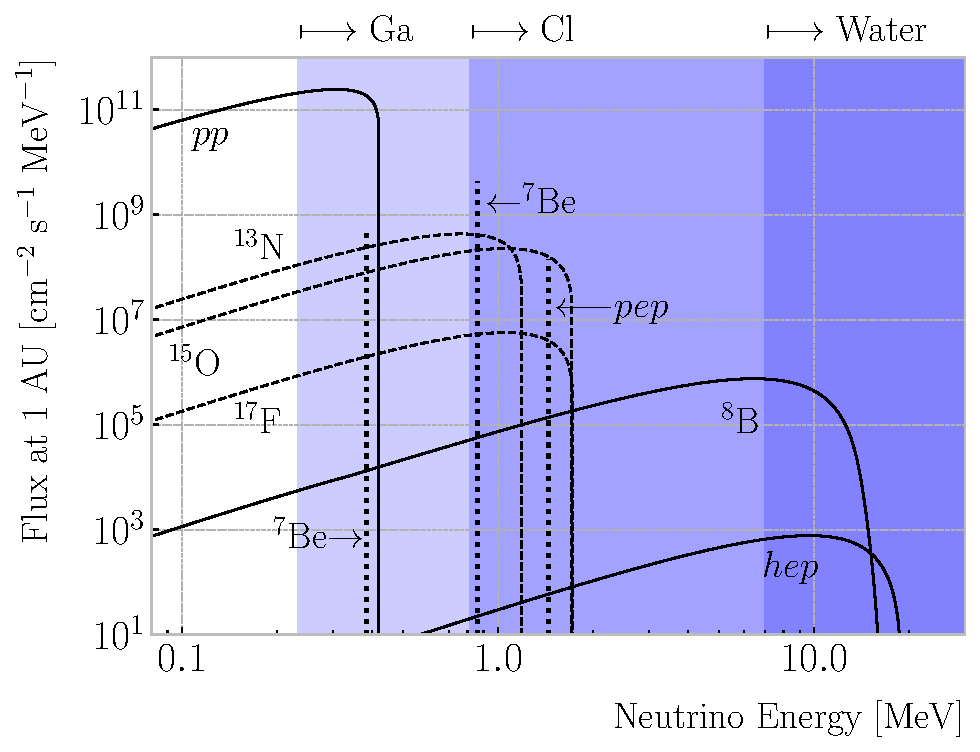
\includegraphics[width=.75\linewidth]{Images/Nu/solar_neutrino_flux.pdf}
	\caption[Solar neutrino fluxes for the solar model BS05(OP).]{Solar neutrino fluxes for the solar model BS05(OP). The detection thresholds for Gallium, Chlorine and water-based experiments are also shown. Figure adapted from Ref. \cite{Bahcall2004}.}
	\label{fig:solar_nu_flux}
\end{figure}

The results of the experiment were compared to the theoretical predictions made by J. Bahcall \cite{Bahcall1968}. During its operation from 1968 to 2002, the experiment observed a solar $\nu_{e}$ flux that was approximately a third of the total prediction \cite{Cleveland1998}.

In the early 1990s, the SAGE \cite{SAGE2009} and GALLEX \cite{GALLEX2010} experiments started operations. The detection principle used for both experiments was similar to that of the Homestake experiment, but using $\prescript{71}{}{\mathrm{Ga}}$ instead of $\mathrm{C}_{2}\mathrm{Cl}_{4}$. With a detection threshold of $0.233~\mathrm{MeV}$, the Gallium-based experiments were able to observe the $pp$ neutrino flux. Both experiments measured a solar electron neutrino flux that was a factor of two lower than the predictions, demonstrating that this deficit was energy-dependent.

In the early 2000s, the SNO experiment put an end to the solar neutrino puzzle \cite{Ahmad2001,Ahmad2002}. Thanks to its directionality capabilities, being a Cherenkov light detector, as well as to its heavy water target, SNO measured the total solar neutrino flux through the NC process:
\begin{equation}
	\nu_{\alpha} + d \longrightarrow n + p + \nu_{\alpha},
\end{equation}
where $\alpha = e, \mu, \tau$. This measurement agreed with the solar model predictions. Then, measuring the CC reaction:
\begin{equation}
	\nu_{e} + d \longrightarrow p + p + e^{-},
\end{equation}
they were able to establish that the $\nu_{\mu}$ and $\nu_{\tau}$ solar fluxes are in fact non-zero, revealing that electron neutrinos were transitioning into different flavours.

\subsection{The atmospheric neutrino problem}

When cosmic-rays interact with the atoms in the upper atmosphere, a plethora of hadrons, mainly $\pi$ and $K$ mesons, are produced. In particular, for the charged pions, we have the following decay chain dominates:
\begin{equation}
	\begin{split}
		&\pi^{+} \longrightarrow \mu^{+} + \nu_{\mu},\\
		&\mu^{+} \longrightarrow e^{+} + \bar{\nu}_{\mu} + \nu_{e},
	\end{split}
\end{equation}
and similar for the antiparticles. For neutrino energies $< 1~\mathrm{GeV}$, the ratio:
\begin{equation}
	\frac{N(\nu_{\mu}+\bar{\nu}_{\mu})}{N(\nu_{e}+\bar{\nu}_{e})},
\end{equation}
of produced neutrinos and antineutrinos is, in good approximation, equal to two \cite{Gaisser2002}.

During the 1980s, several proton decay experiments, like Kamiokande \cite{Hirata1988}, IMB \cite{Casper1991}, MACRO \cite{Ambrosio1998}, and Soudan-2 \cite{Allison1997}, measured the flux of atmospheric neutrinos. This was an important part of their research programme, as the atmospheric neutrinos constitute their main background. All these experiments reported an atmospheric neutrino ratio lower than the predictions.

\begin{figure}[t]
	\centering
	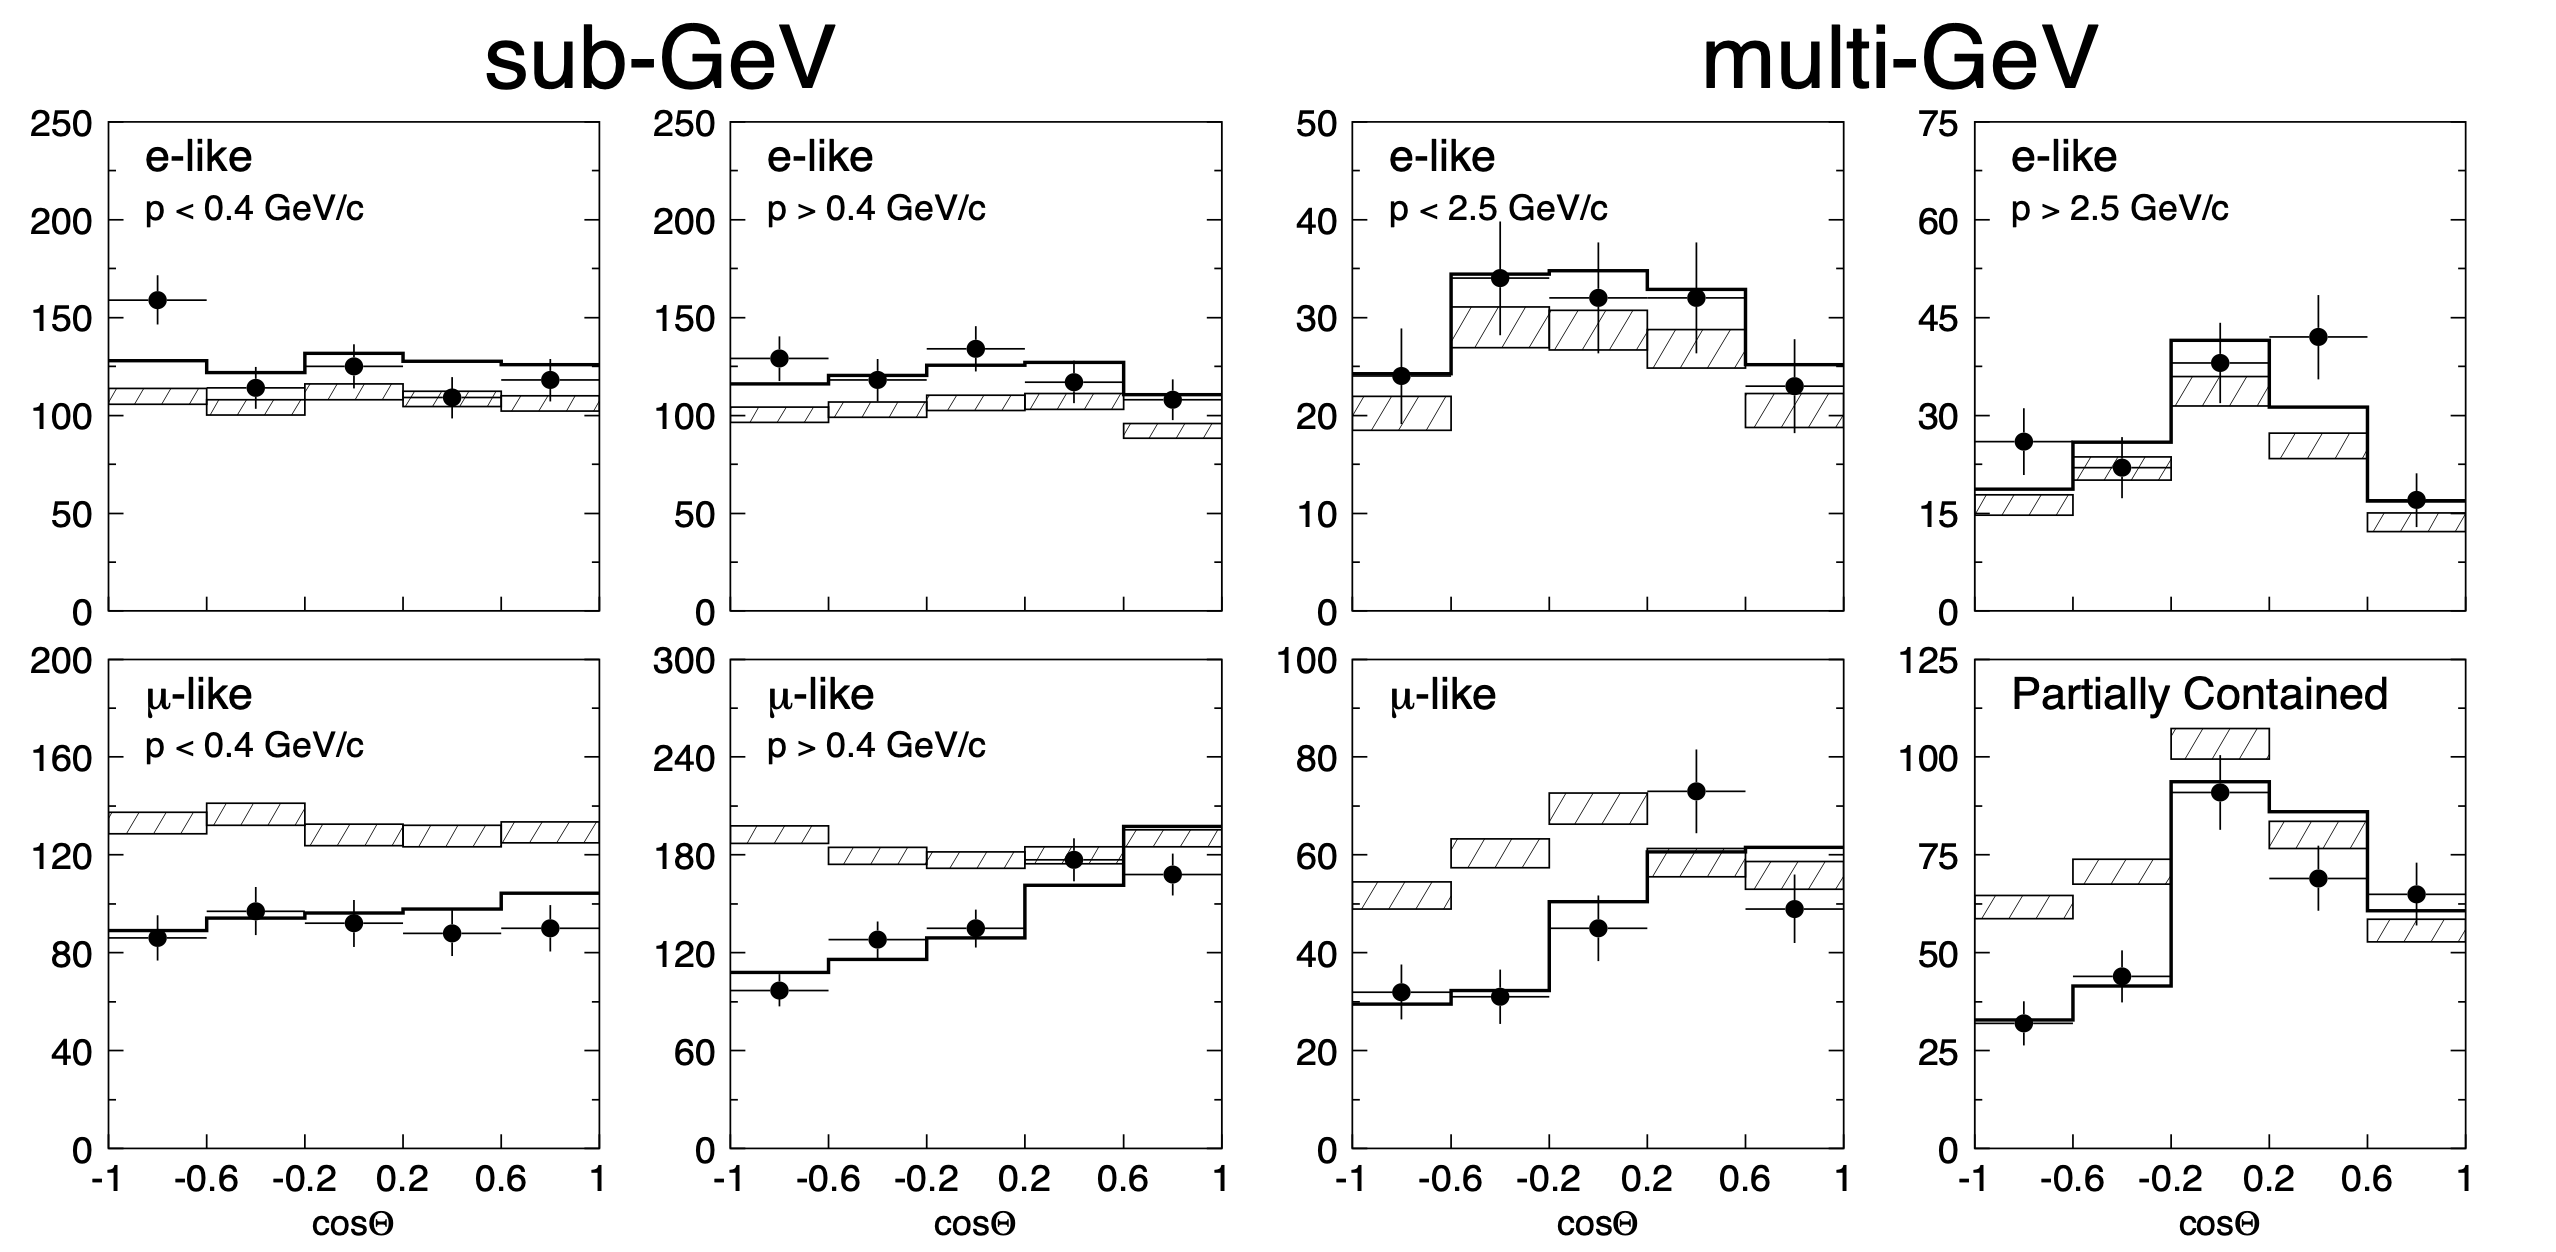
\includegraphics[width=.90\linewidth]{Images/Nu/superk_oscillations.png}
	\caption[Zenith angle distributions for the selected $\nu_{e}$ and $\nu_{\mu}$ events in the SK detector.]{Zenith angle distributions for the selected $\nu_{e}$ (top row) and $\nu_{\mu}$ (bottom row) events in the SK detector. The hatched region corresponds to the expectation in the case of no oscillations, whereas the solid line indicates the best-fit in the case of $\nu_{\mu} \rightarrow \nu_{\tau}$ oscillations. Figure taken from Ref. \cite{SuperKamiokande1998}.}
	\label{fig:atmospheric_nu_osc}
\end{figure}

A few years before the SNO discovery, in 1998, Super-Kamiokande (SK) collaboration measured the atmospheric $\nu_{e}$ and $\nu_{\mu}$ spectra as a function of the zenith angle \cite{SuperKamiokande1998}. Upward-going particles have negative zenith angle, $\mathrm{cos}~\Theta < 0$, indicating that they entered from the bottom of the detector. These upward-going neutrinos had to travel through the Earth in order to reach the detector, allowing SK to probe a broad range of baselines. Figure \ref{fig:atmospheric_nu_osc} shows the reported distributions (black dots), compared to the no oscillations prediction (hatched region). This measurement confirmed that muon neutrinos transition to other flavours, and that this phenomenon depends both on the energy and the path length of the neutrino.

The SK and SNO findings provided definitive evidence for the existence of neutrino oscillations, and therefore non-zero neutrino masses. This constitutes one of the groundbreaking discoveries of modern physics and has acted as driving force for beyond the Standard Model (BSM) physics. The minimal extension of the SM we can do to address these phenomena is introducing different masses for at least two of the neutrinos. This way, we are left with three neutrino mass eigenstates $\nu_{1}$, $\nu_{2}$, and $\nu_{3}$, with masses $m_{1}$, $m_{2}$, and $m_{3}$ respectively, which in general will not coincide with the flavour eigenstates, $\nu_{e}$, $\nu_{\mu}$, and $\nu_{\tau}$.

\section{Massive neutrinos}

The existence of neutrino oscillations imply that neutrinos are massive particles. However, as we have seen before, within the SM neutrinos are massless, as they do not have a mass term in the Lagrangian. If one wants to give neutrinos a mass, the particle content of the SM needs to be expanded.

A way of generating massive neutrinos while maintaining gauge invariance is by introducing an arbitrary number of sterile neutrinos $N_{i}$, $i=1,\dots,m$. These allow for two different types of neutrino mass terms:
\begin{equation}\label{2.10}
	-\mathcal{L}_{M_{\nu}} = \sum_{i=1}^{m} \sum_{j=1}^{3} M^{ij}_{D} \bar{N}_{i} \nu_{Lj} + \frac{1}{2} \sum_{i=1}^{m} \sum_{j=1}^{m} M^{ij}_{N} \bar{N}_{i} N^{c}_{j} + \mathrm{h.c.},
\end{equation}
where $M_{D}$ is a complex $m \times 3$ matrix and $M_{N}$ a complex and symmetric $m \times m$ matrix. The first term, often referred to as the Dirac mass term, arises from the corresponding Yukawa interaction after the spontaneous electroweak symmetry breaking, similar to the other fermions. The second term, called the Majorana mass term, is allowed in the Lagrangian, as it is a singlet of the gauge group. However, it violates lepton number conservation by two units.

If one imposes lepton number symmetry conservation, the Majorana term must banish, $M_{N}=0$. In this case, if $m=3$ we can identify the sterile neutrinos as the right-handed component of the neutrino field. The Dirac mass matrix can be diagonalised using two unitary matrices, $V^{\nu}_{R}$ and $V^{\nu}_{L}$, as:
\begin{equation}
	M_{D} = V^{\nu}_{R}~\mathrm{diag}(m_{1}, m_{2}, m_{3})~V^{\nu \dagger}_{L},
\end{equation}
where $m_{i}$, $i=1,2,3$ are the masses of the three neutrino mass eigenstates.

The neutrino mass term can be written in term of the resulting eigenstates as:
\begin{equation}
	-\mathcal{L}_{M_{\nu}} = \sum_{i=1}^{3} m_{i}~\bar{\nu}_{Di} \nu_{Di},
\end{equation}
with:
\begin{equation}
	\nu_{Di} = \left(V^{\nu \dagger}_{L}~\nu_{L}\right)_{i} + \left(V^{\nu \dagger}_{R}~N\right)_{i}.
\end{equation}

In this scenario, both the low energy particle budget and the symmetries of the SM have to be modified. Moreover, the masses of the neutrinos are generated exclusively through the Higgs mechanism, which does not explain why they are much smaller than those of the charged leptons.

Going back to the general case, we can re-write Eq. (\ref{2.10}) in matrix form as:
\begin{equation}
	-\mathcal{L}_{M_{\nu}} = \frac{1}{2} \begin{pmatrix}\bar{\nu}^{c}_{L},&\bar{N}\end{pmatrix} \begin{pmatrix}0 & M_{D}^{T}\\M_{D} & M_{N}\end{pmatrix}\begin{pmatrix}\nu_{L}\\N^{c}\end{pmatrix} + \mathrm{h.c.} = \bar{\nu}^{c} M_{\nu} \nu + \mathrm{h.c.},
\end{equation}
with $\nu=\begin{pmatrix}\nu_{L}, & N^{c}\end{pmatrix}^{T}$ being a $(3+m)$-dimensional vector grouping the active and the sterile neutrinos. The matrix $M_{\nu}$, which is a complex $(3+m)\times(3+m)$ symmetric matrix, can be diagonalised by means of a unitary matrix $V^{\nu}$, yielding:
\begin{equation}
	M_{\nu} = V^{\nu}~\mathrm{diag}(m_{1}, m_{2}, \dots, m_{3+m})~V^{\nu T}.
\end{equation}

Using this eigendecomposition, the neutrino mass term can be expressed as:
\begin{comment}
\begin{equation}
	\begin{split}
		-\mathcal{L}_{M_{\nu}} &= \frac{1}{2} \sum_{i=1}^{3+m} m_{i} \left[\left(\vphantom{V^{\nu \dagger}}\bar{\nu}^{c}~V^{\nu}\right)_{i} \left(V^{\nu \dagger}~\nu\right)_{i} + \left(\vphantom{V^{\nu \dagger}}\bar{\nu}~V^{\nu}\right)_{i} \left(V^{\nu \dagger}~\nu^{c}\right)_{i}\right]\\
		&= \frac{1}{2} \sum_{i=1}^{3+m} m_{i}~\bar{\nu}_{M i} \nu_{M i},
	\end{split}
\end{equation}
\end{comment}
\begin{equation}
	-\mathcal{L}_{M_{\nu}} = \frac{1}{2} \sum_{i=1}^{3+m} m_{i}~\bar{\nu}_{M i} \nu_{M i},
\end{equation}
where the states $\nu_{M i}$, commonly referred to as Majorana neutrinos, are defined as:
\begin{equation}
	\nu_{M i} = \left(V^{\nu\dagger}~\nu\right)_{i} + \left(V^{\nu\dagger}~\nu\right)^{c}_{i},
\end{equation}
in such a way that the Majorana condition, $\nu^{c}_{M} = \nu_{M}$, holds true.

As a consequence of the Majorana condition, the neutrino and the antineutrino states can be described in terms of a single field. As opposed to the charged leptons, which need to be represented by a four-component or Dirac spinor, the Majorana neutrino is described by a two-component or Weyl spinor.

If the eigenvalues of the Majorana mass matrix, $M_{N}$, are much larger than the electroweak symmetry breaking scale, the diagonalisation of $M_{\nu}$ leads to $3$ light and $m$ heavy neutrino states:
\begin{equation}
	-\mathcal{L}_{M_{\nu}} = \frac{1}{2} \bar{\nu}_{l} M_{l} \nu_{l} + \frac{1}{2} \bar{\nu}_{h} M_{h} \nu_{h},
\end{equation}
where the two mass matrices are given by:
\begin{equation}
	\begin{split}
		M_{l} &\simeq -V_{l}^{T} M_{D}^{T} M_{N}^{-1} M_{D} V_{l},\\
		M_{h} &\simeq V_{h}^{T} M_{N} V_{h},
	\end{split}
\end{equation}
with $V_{l}$ and $V_{h}$ two unitary matrices.

This scenario represents the so-called see-saw mechanism.

\section{Neutrino oscillation formalism}

The way to relate these two sets of neutrino eigenstates is via a $3 \times 3$ unitary matrix, called the Pontecorvo-Maki-Nakagawa-Sakata (PMNS) matrix \cite{Pontecorvo1957, Maki1962}, as:
\begin{equation}\label{2.1}
\ket{\nu_{\alpha}} = \sum_{i=1}^{3} U^{*}_{\alpha i} \ket{\nu_{i}},
\end{equation}
where the Greek index $\alpha$ denotes the flavour $\{e,\mu,\tau\}$ and the Latin index $i$ the associated masses $\{1,2,3\}$. This leptonic mixing matrix may be parametrized in terms of 6 parameters, 3 of which are mixing angles $\theta_{12}$, $\theta_{13}$ and $\theta_{23}$, one CP-violating phase $\delta_{CP}$ and 2 Majorana phases $\alpha$ and $\beta$:
\begin{equation}\label{2.2}
U = \left(\begin{array}{ccc}1&0&0\\0&c_{23}&s_{23}\\0&-s_{23}&c_{23}\end{array}\right) \left(\begin{array}{ccc}c_{13}&0&s_{13} \mathrm{e}^{-i\delta_{CP}}\\0&1&0\\-s_{13} \mathrm{e}^{-i\delta_{CP}}&0&c_{13}\end{array}\right) \left(\begin{array}{ccc}c_{12}&s_{12}&0\\-s_{12}&c_{12}&0\\0&0&1\end{array}\right) \left(\begin{array}{ccc}1&0&0\\0&\mathrm{e}^{i\alpha}&0\\0&0&\mathrm{e}^{i\beta}\end{array}\right),
\end{equation}
where $c_{ij} \equiv \cos \theta_{ij}$ and $s_{ij} \equiv \sin \theta_{ij}$. This matrix is analogous to the Cabibbo-Kobayashi-Maskawa (CKM) matrix in the quark sector. If neutrinos are Dirac fermions, we can drop the Majorana phases in the PMNS matrix. But, in any case, these phases play no role on the neutrino oscillations.

\subsection{Oscillations in vacuum}

Consider the case where a neutrino of flavour $\alpha$ is produced at $t=0$, and then it propagates through vacuum. Such a state will evolve in time according to the relation:
\begin{equation}\label{2.3}
\ket{\nu_{\alpha}(t)} = \sum_{i=1}^{3} U^{*}_{\alpha i} \mathrm{e}^{-iE_{i}t} \ket{\nu_{i}(t=0)},
\end{equation}
as the mass eigenstates are also eigenstates of the free Hamiltonian. Now, if we express the mass eigenstates as a superposition of flavour eigenstates, the last expression can be rewritten as:
\begin{equation}\label{2.4}
\ket{\nu_{\alpha}(t)} = \sum_{i=1}^{3} U_{\beta i} \mathrm{e}^{-iE_{i}t} U^{*}_{\alpha i} \ket{\nu_{\beta}}.
\end{equation}

This way, the probability for the neutrino to transition from flavour $\alpha$ to flavour $\beta$ will be given by:
\begin{equation}\label{2.5}
P(\nu_{\alpha} \rightarrow \nu_{\beta}) = \left|\braket{\nu_{\beta}}{\nu_{\alpha}(t)}\right|^{2}=\left|\sum_{i=1}^{3} U_{\beta i} \mathrm{e}^{-iE_{i}t} U^{*}_{\alpha i}\right|^{2}.
\end{equation}

A usual approximation to take at this point is to consider ultra-relativistic neutrinos, i.e. $E \approx \left|\vec{p}\right|$, so we can write the dispersion relations as:
\begin{equation}\label{2.6}
E_{i} = \sqrt{p^{2} + m_{i}^{2}} \approx E + \frac{m_{i}^{2}}{2 E},
\end{equation}
so we can write the oscillation probability as:
\begin{equation}\label{2.7}
\begin{split}
P(\nu_{\alpha} \rightarrow \nu_{\beta}) &= \sum_{i,j} U^{*}_{\alpha i} U_{\beta i} U_{\alpha j} U^{*}_{\beta j} \mathrm{e}^{-i\frac{\Delta m^{2}_{ij}}{2E}t}\\
&=\delta_{\alpha\beta} - 4 \sum_{i<j} \mathfrak{Re}\left[U^{*}_{\alpha i} U_{\beta i} U_{\alpha j} U^{*}_{\beta j}\right] \sin^{2}\left(\frac{\Delta m^{2}_{ij}}{4E}t\right)\\
&\phantom{=}+ 2  \sum_{i<j} \mathfrak{Im}\left[U^{*}_{\alpha i} U_{\beta i} U_{\alpha j} U^{*}_{\beta j}\right] \sin\left(\frac{\Delta m^{2}_{ij}}{2E}t\right),
\end{split}
\end{equation}
where $\Delta m^{2}_{ij}$ is the difference of the squared masses of the $j$th and $i$th neutrino mass eigenvalues. At this point, it is usual to write the phase responsible for the oscillations as (under the approximate assumption $t \approx L$):
\begin{equation}\label{2.8}
\Delta_{ij} \equiv \frac{\Delta m^{2}_{ij}}{4E}L \simeq 1.27 \frac{\Delta m^{2}_{ij}}{(\mathrm{eV}^{2})} \frac{L}{(\mathrm{km})} \frac{(\mathrm{GeV})}{E}.
\end{equation}

Notice that, in the case of antineutrinos the only difference would be the sign of the last term in the oscillation probability. This way, one can write the CP asymmetry as:
\begin{equation}\label{2.9}
\begin{split}
A^{\alpha\beta}_{CP}&=P(\nu_{\alpha} \rightarrow \nu_{\beta})-P(\bar{\nu}_{\alpha} \rightarrow \bar{\nu}_{\beta})\\
&=4  \sum_{i<j} \mathfrak{Im}\left[U^{*}_{\alpha i} U_{\beta i} U_{\alpha j} U^{*}_{\beta j}\right] \sin 2\Delta_{ij}.
\end{split}
\end{equation}

\subsection{Oscillations in matter}

When neutrinos propagate through matter, their oscillation can be affected in mainly two ways. First, neutrinos can inelastically scatter with nuclei, thus destroying the coherent propagation of their quantum state. Nevertheless, in most cases this effect is negligible (even in very dense mediums like the core of the Sun). Second, neutrinos can also experience coherent or forward scatterings, that can affect their oscillation but not lose the coherent propagation of the state.

The first proposed model to account for neutrino oscillations in matter was proposed by Mikhaev, Smirnov and Wolfenstein (MSW) \cite{Wolfenstein1977}. It relies on the fact that, as the only charged lepton present in ordinary matter is the electron, electron neutrinos can undergo both charged and neutral-current interactions with matter whereas for muon and tau neutrinos just neutral currents are possible.

\subsection{Current status of neutrino oscillations}

A wide range of neutrino experiments provide experimental input to the neutrino oscillation framework, both using natural or synthetic neutrino sources. The results from one of the neutrino global fit analyses, shown in Tab. \ref{tab:neutrino_global_fit} \footnote{These are the results reported during M. T\'{o}rtola's talk at Neutrino 2024 (see this \href{https://agenda.infn.it/event/37867/contributions/233956/attachments/121839/178002/MTortola-Neutrino2024.pdf}{link}). I need to keep an eye and see if they publish these or other updated results in the near future.}, summarise well our current understanding of the different oscillation parameters.

\textbf{Solar neutrino experiments} detect neutrinos produced in thermonuclear reactions inside the Sun, mainly from the so-called $pp$ chain and the CNO cycle. These neutrinos have a typical energy in the range from $0.1$ to $20 \ \mathrm{MeV}$. These experiments (Homestake \cite{Homestake1998}, GALLEX \cite{GALLEX2010}, SAGE \cite{SAGE2009}, Borexino \cite{Borexino2011}, Super-Kamiokande \cite{Super-Kamiokande2005} and SNO \cite{SNO2011}) provide the best sensitivities to $\theta_{12}$ and $\Delta m^{2}_{21}$.

\textbf{Atmospheric neutrino experiments} detect the neutrino flux produced when cosmic rays scatter with particles in Earth's atmosphere. These collisions generate particle showers that eventually produce electron and muon neutrinos (and antineutrinos). Their energies range from few $\mathrm{MeV}$ to about $10^{9} \ \mathrm{GeV}$. Experiments, like Super-Kamiokande \cite{Super-Kamiokande2017} and IceCube \cite{IceCube2017} use atmospheric neutrinos to measure oscillations and are specially sensitive to $\theta_{23}$ and $\Delta m^{2}_{32}$.

\textbf{Reactor neutrino experiments} look for the $\bar{\nu}_{e}$ spectrum produced by nuclear reactors, with energies in the $\mathrm{MeV}$ scale. Depending on the distance to the source, long-baseline experiments like KamLAND \cite{KamLAND2013} are sensitive to the solar mass splitting $\Delta m^{2}_{21}$ whereas much shorter baseline experiment such as RENO \cite{RENO2018} or DayaBay \cite{DayaBay2018} measure $\theta_{13}$ and $\Delta m^{2}_{31}$.

\textbf{Accelerator experiments} measure neutrino fluxes generated in particle accelerators. Usually mesons are produced in the accelerator to be focused into a beam, then some decay to muon neutrinos and the rest are absorbed by a target. Depending on the configuration one can obtain a beam made of mostly neutrinos or antineutrinos. The typical energies of these neutrinos are in the $\mathrm{GeV}$ range. Experiments such as NOvA \cite{Nova2020}, T2K \cite{T2K2020}, MINOS \cite{MINOS2014}, OPERA \cite{OPERA2018} and K2K \cite{K2K2006} (and in the future DUNE \cite{DUNE2020}) are primarily sensitive to $\theta_{13}$, $\theta_{23}$ and $\Delta m^{2}_{32}$. Also, in the coming years  DUNE \cite{DUNE2020} and Hyper-Kamiokande \cite{Hyper-Kamiokande2019} will be sensitive to $\delta_{CP}$.

\begin{table}
\centering
\caption{Summary of neutrino oscillation parameters determined in the Neutrino Global Fit of 2020 \cite{deSalas2020}.}
	\begin{tabular}{c|c|c}
		Parameter                                               & Best fit $\pm ~ 1\sigma$ & $3 \sigma$ range   \\[1mm] \hline \rule{0pt}{1.1\normalbaselineskip}
		$\Delta m^{2}_{21}~[\mathrm{eV}^{2} \times 10^{-5}]$                   & $7.55^{+0.22}_{-0.20}$ & $6.98-8.19$\\[3mm]
		$\left|\Delta m^{2}_{31}\right|~[\mathrm{eV}^{2}\times 10^{-3}]$ (NO) & $2.51^{+0.02}_{-0.03}$    & $2.43-2.58$\\[2mm]
		$\left|\Delta m^{2}_{31}\right|~[\mathrm{eV}^{2}\times 10^{-3}]$ (IO) & $2.41^{+0.03}_{-0.02}$ & $2.34-2.49$    \\[3mm]
		$\sin^{2} \theta_{12} / 10^{-1}$ & $3.04 \pm 0.16$ & $2.57-3.55$ \\[3mm]
		$\sin^{2} \theta_{23} / 10^{-1}$ (NO) & $5.64^{+0.15}_{-0.21}$ & $4.23-6.04$ \\[2mm]
		$\sin^{2} \theta_{23} / 10^{-1}$ (IO) & $5.64^{+0.15}_{-0.18}$ & $4.27-6.03$ \\[3mm]
		$\sin^{2} \theta_{13} / 10^{-2}$ (NO) & $2.20^{+0.05}_{-0.06}$ & $2.03-2.38$ \\[2mm]
		$\sin^{2} \theta_{13} / 10^{-2}$ (IO) & $2.20^{+0.07}_{-0.04}$ & $2.04-2.38$ \\[3mm]
		$\delta_{CP} / \pi$ (NO) & $1.12^{+0.16}_{-0.12}$ & $0.76-2.00$ \\[2mm]
		$\delta_{CP} / \pi$ (IO) & $1.50^{+0.13}_{-0.14}$ & $1.11-1.87$
	\end{tabular}
	\label{tab:neutrino_global_fit}
\end{table}

\section{Open questions in the neutrino sector}

A crucial question that remains open these days, and is of vital importance for oscillation phenomena, is whether the mass eigenvalue $\nu_{3}$ is the heaviest (what we call normal ordering) or the lightest (refered to as inverted ordering) of the mass eigenstates. In other words, this means that we do not know the sign of $\Delta m^{2}_{32}$, so we can either have $m_{1}<m_{2}<m_{3}$ (NO) or $m_{3}<m_{1}<m_{2}$ (IO).

Another big puzzle is related to the value of $\delta_{CP}$. Nowadays it is poorly constrained, with all values between $\pi$ and $2\pi$ being consistent with data. A prospective measurement different from $\delta_{CP}=0,\pi$ will predict CP-violation in the leptonic sector, and thus contribute along with the one measured in the quark sector to the total amount of CP-violation. Although it is true that these two contributions by themselves are not enough to explain the matter anti-matter asymmetry in our universe, the amount of CP-violation in the leptonic sector can be key to explain such imbalance.

Both of these questions, because of their nature, could be understood thanks to future oscillation experiments.

Notwithstanding, there are other mysteries that can not be unveiled just by conducting oscillation experiments, as certain quantities do not influence these phenomena. Among these there is the question of the absolute values of the neutrino masses. Depending on the value of the lightest of the neutrino masses we can have different mass spectra, from hierarchical $m_{1} \ll m_{2}<m_{3}$ (NO) or $m_{3} \ll m_{1}<m_{2}$ (IO) to quasi-degenerate $m_{1} \simeq m_{2} \simeq m_{3}$.

Other open question concerns the nature itself of the neutrinos. If neutrinos are Dirac particles then their mass term can be generated through the usual Higgs mechanism by adding right-handed neutrino fields. However, if they are Majorana particles and therefore their own antiparticles, there is no need to add extra fields to have the mass term in the Lagrangian. Experiments like SuperNEMO \cite{SuperNEMO2010}, SNO+ \cite{SNO2015} and NEXT \cite{NEXT2020}, which search for neutrino-less double beta decay, will be able to determine whether neutrinos are Dirac or Majorana.

\section{Neutrino interactions}

\begin{figure}[t]
	\begin{subfigure}{0.5\textwidth}
		\centering
		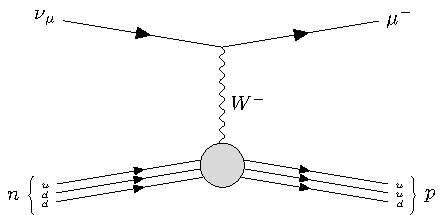
\includegraphics[width=.90\linewidth]{Images/Nu/feynman_ccqel.pdf}
	\end{subfigure}
	\begin{subfigure}{0.5\textwidth}
		\centering
		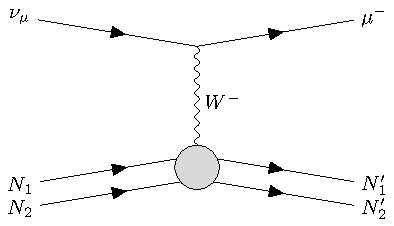
\includegraphics[width=.90\linewidth]{Images//Nu/feynman_ccmec.pdf}
	\end{subfigure}
	\begin{subfigure}{0.5\textwidth}
		\centering
		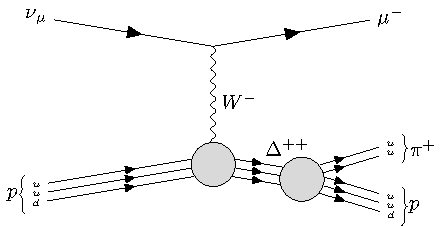
\includegraphics[width=.90\linewidth]{Images//Nu/feynman_ccres.pdf}
	\end{subfigure}
	\begin{subfigure}{0.5\textwidth}
		\centering
		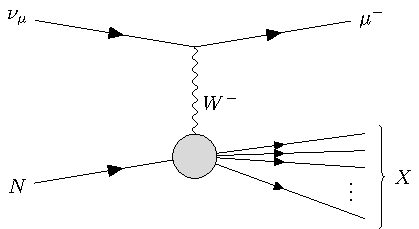
\includegraphics[width=.90\linewidth]{Images//Nu/feynman_ccdis.pdf}
	\end{subfigure}
	\caption{}
	\label{fig:neutrino_cc_interactions}
\end{figure}

\begin{figure}[t]
	\centering
	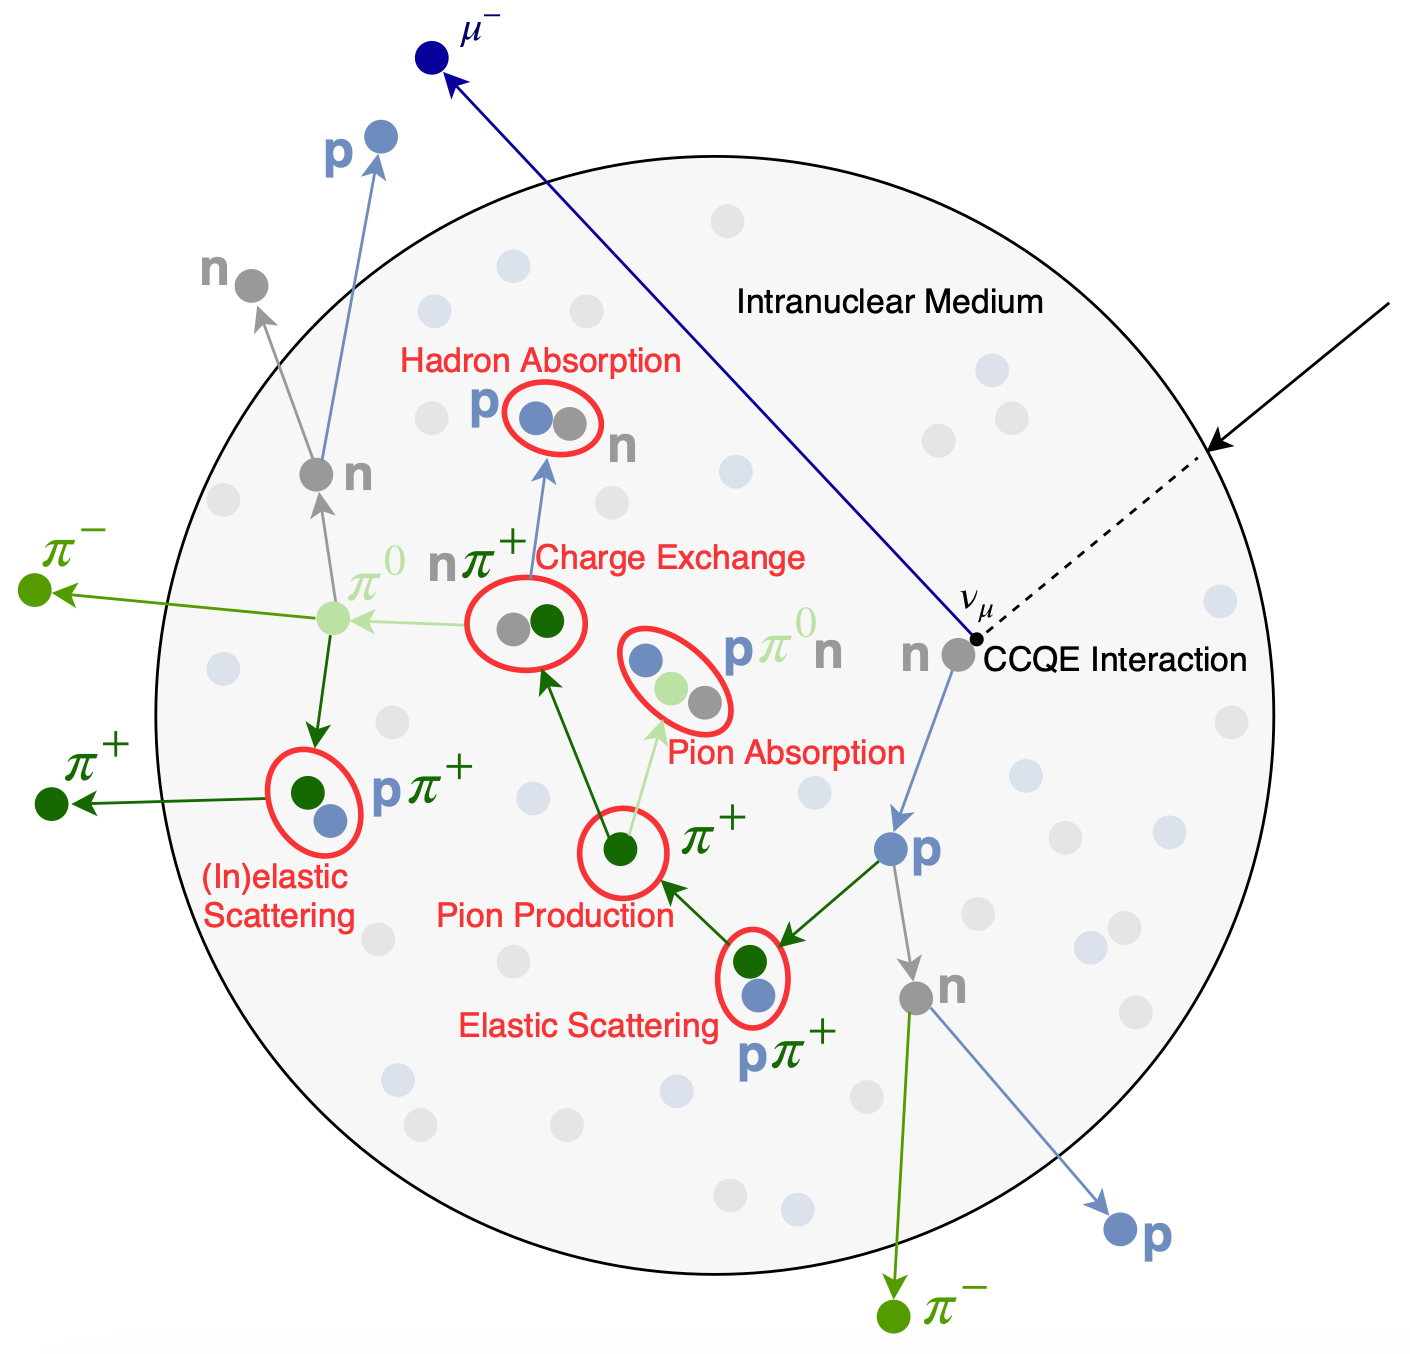
\includegraphics[width=.55\linewidth]{Images/Nu/lars_fsi.png}
	\caption[Schematic representation of a $\nu_{\mu}$ CCQE interaction with a neutron inside a nucleus.]{Schematic representation of a $\nu_{\mu}$ CCQE interaction with a neutron inside a nucleus. The reaction produces a muon and a proton, which travel through the nuclear medium. The outgoing proton undergoes various kinds of hadronic FSIs on its way out. Figure taken from Ref. \cite{Bathe-Peters2022}.}
	\label{fig:fsi_diagram}
\end{figure}